% \section{System Testing and Verification}
% In this chapter, you have to explain all the steps you carried out to ensure that project outcomes are realized correctly. Your testing setup, strategy and environment should therefore be described. Your efforts for unit testing as well as integrated system testing should be given. Finally, the results from different testing scenarios should be highlighted and discussed. 

% In this space, before the first section, write an introductory paragraph on how you test and verify the correct operation of your system

In this chapter we present all of our journey and the steps that led to every single decision that we made concerning each of the models (agents) and the system as a whole. This chapter goes as follows: first we start by describing our plan from the start, and how we came with it \ref{sec:setup}, then we delve into the fine details of creating, tuning, evaluating and testing each module \ref{sec:plan}, comparing each one of them with its benchmark.



\section{Testing Setup}
\label{sec:setup}
We divided our project into two main separate components: 1- \textbf{AI agents}, 2- \textbf{web application}. AI agents consist of three models (agents), each one of them was tested individually and compared against a state of the art application tackling the same problem with different approach (architecture). Web application was build independently as well, tested and verified. Then we merged these two components and tested their performance as a whole.

AI agents does not communicate, so we were able to test each one of them separately. As we mentioned before, to conquer our problem statement we distributed the work load among several machines, so in order to make a proof of work of our approach and implementation we tested the system with and without distributing load and compared results \ref{sec:integration_test}.


\section{Testing Plan and Strategy}
\label{sec:plan}
Our strategy for each agent was the same; first we build an agent with a pre-trained model, tune and test it to accomplish the best results there is, then we build our own models and compare it against our ground truth (highest roof).\\

For integration testing, we first validated that the application works properly without distribution of the work load (ie. normal web application), feeding it one model at a time, then configure it to work with multiple nodes on one machine, and finally distributing it among different machines. For the rest of this section we discuss the steps that led to every decision and improvement to each of our modules, comparing them with their benchmarks, and conclude our discussion with the whole system's testing and verification process.\\

Please notice that \textit{front-end} is a huge module that was built independently, and tested manually (while implementing it with no frameworks), so we didn't add its specifications in this chapter, rather than that we provided Appendix B entirely for the purpose of displaying front-end and its functionalities.




\newpage
\subsection{Module Testing 1: Emotion Detection Agent}
\label{sec:emotion_testing}
Please refer to module's introduction at section: \ref{sec:module_1} before going deeper in this section!\\

\textbf{Dataset}: No problem found when searching for a dataset appropriate to our task, as a matter of fact the problem of emotion detection is widely known since 2012 (or earlier). \href{https://www.kaggle.com/c/challenges-in-representation-learning-facial-expression-recognition-challenge/data}{\underline{Fer2013}} dataset was the only dataset needed for training and testing our architecture.\\

\textbf{Pre-trained model (ground truth)}: We used transfer learning \ref{Transfer Learning} to create our ground truth model, using VGG16 model (pre-trained) figure \ref{fig:cnn_1} to extract features from images, and then trained two fully connected layers following it, first one reduces the output number of features by 4, and the second one used for prediction. Dimensions evolve as follows: 1- images are $[48 \times 48 \times 1]$, transformed into $[224 \times 224 \times 3]$ to fit VGG16, 2- features extracted from VGG16 are $[1000]$, 3- first fully-connected layer transform it into $[250]$ followed by ReLU activation function, and  4- second fully-connected layer responsible for prediction returns $[7]$ outputs, one for each class, followed by soft-max function for normalizing the outputs.\\

\textbf{Tuning}: Dataset was quite large, so tuning on local machines was not feasible; it took nearly 3 hours to run one epoch, so we let it run for three consecutive days until the program crashed. Then we realised that in order to tune our hyperparameters we need to train and test on a smaller subset of data, so we did so on 0.01\% of data, and came up with the following hyperparameters.\\

\textbf{Training settings}: We were aware of the massive size of the model in hand so we didn't train the pre-trained part of the model, instead we kept as is. Training only the last two fully connected layers. Splitted the dataset into 80\% training and 20\% validation (testing). Trained using \textit{Adam} optimization function with learning rate equals 0.001, added learning rate \textit{scheduler}; to decrease it as training goes further, and \textit{cross-entropy} loss function. Trained for 100 epochs, using \href{https://aws.amazon.com/}{AWS} (Amazon web services), with a \textit{P2} instance (provided with a high GPU quota) for nearly 10 hours.\\

\textbf{Results 1}: Considering figure: \ref{fig:emoiton_result_1}, we can see that after epoch number 30 the model overfits validation subset of data, even though it was very large, but the complexity of VGG16 overcame it and was able to overfit. However, final results (when provided with a video) was quite impressive and did exactly the required job.\\


\begin{figure}[h!]
\centering
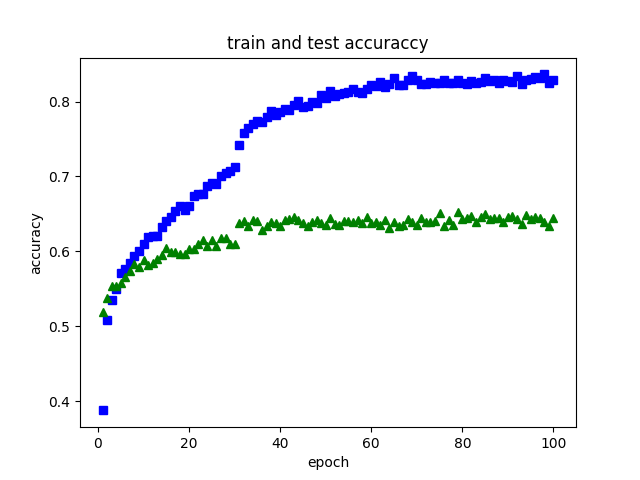
\includegraphics[width=0.8\textwidth]{images/emotion_result_1.png}
\caption{Pre-trained model train/validate accuracy}
\label{fig:emoiton_result_1}
\end{figure}

\textbf{Merging}: We merged the image-based model to be able to process videos and manually test the pre-trained model with real-life examples. \\

\textbf{Testing manually}: Finally we tested on a real example, a stand-up-comic \href{https://drive.google.com/file/d/1EWS8MHNyOIC2-ZVFIYlGsj9iM1l3pnp5/view?usp=sharing}{\underline{video}}, for a man telling jokes, tested for the first one minute (ie. 1800 frames). Processing the first minute of the video took nearly 3.5 minutes, which was unacceptable; because we aim to ease the processing time for interviewers and of course this implies being able to act/process faster. Nevertheless, results was very acceptable and accurately correct.\\

\textbf{Intuition}: We came to a realization that we needed a simpler model, that performs nearly the same (or better) than our ground truth, and operates faster, without the problem overfitting.\\

\textbf{Actual model}: After a long time surfing and reading related articles and papers, we came across a very simple architecture \cite{ariaga} yet a powerful one. That used two new techniques in ANN; residual neural network and depth-wise separable convolution. We implemented it right away, and tuned it to be suitable for our dataset.\\

\textbf{Tuning}: The model was small -relatively- so we were able to tune it as much as we wanted to see table: \ref{tbl:emotion_tune}, since training one epoch with the whole dataset on CPU takes $3$ minutes maximum. We started tuning the size of our architecture, tried four different sizes, and finally settled with four (residual neural network with depth-wise separable convolution). Then, we tuned the learning rate hyperparameter. Initially when we were tuning the architecture size we used the default value for learning rate with adam optimizer (0.0001). Each test took about an hour, running for (30 to 50) epochs with batch size = 32, trained on CPU.\\


\begingroup
\centering
\begin{tabular} { | p {5 cm} | p {2 cm} || p {5 cm} |p {2 cm} |}
    \hline
    \textbf{Tune} & \textbf{Val accuracy} & \textbf{Architecture} & \textbf{Val accuracy}\\
    \hline
    
    \hline
    \rule{0pt}{15pt} learning rate=0.1 &  0.3 & 1 residual and depth-wise & 0.38\\
    \hline
    \rule{0pt}{15pt} learning rate=0.01 &  0.62 & 2 residual and depth-wise & 0.36\\
    \hline
    \rule{0pt}{15pt} learning rate=0.001 &  0.66 & 3 residual and depth-wise & 0.57\\
    \hline
    \rule{0pt}{15pt} learning rate=0.0001 &  0.49 & 4 residual and depth-wise & 0.67\\
    \hline
    
    
\end{tabular}
\captionof{table}{Tuning trained model}
\label{tbl:emotion_tune}
\endgroup
\vspace{1cm}



\textbf{Final training settings}: As usual we used adam optimizer, cross-entropy loss, and L2 regularization. Tuned hyperparameters are as follows:
\begin{itemize}
    \item batch size: 32
    \item learning rate: 0.001
    \item L2 regularization lambda: 0.01\\
\end{itemize}

\textbf{Results 2}: Considering figure: \ref{fig:emoiton_results_2}, validation (test) accuracy saturates after epoch: 60, however this is not considered as overfitting; because training accuracy also saturates at that level, looking at losses figure: \ref{fig:emoiton_loss_2} we can see that after epoch: 60 training loss is not decreasing (ie. saturating at convergence).\\


\begin{figure}
    % \centering
    \begin{subfigure}[b]{0.5\textwidth}
        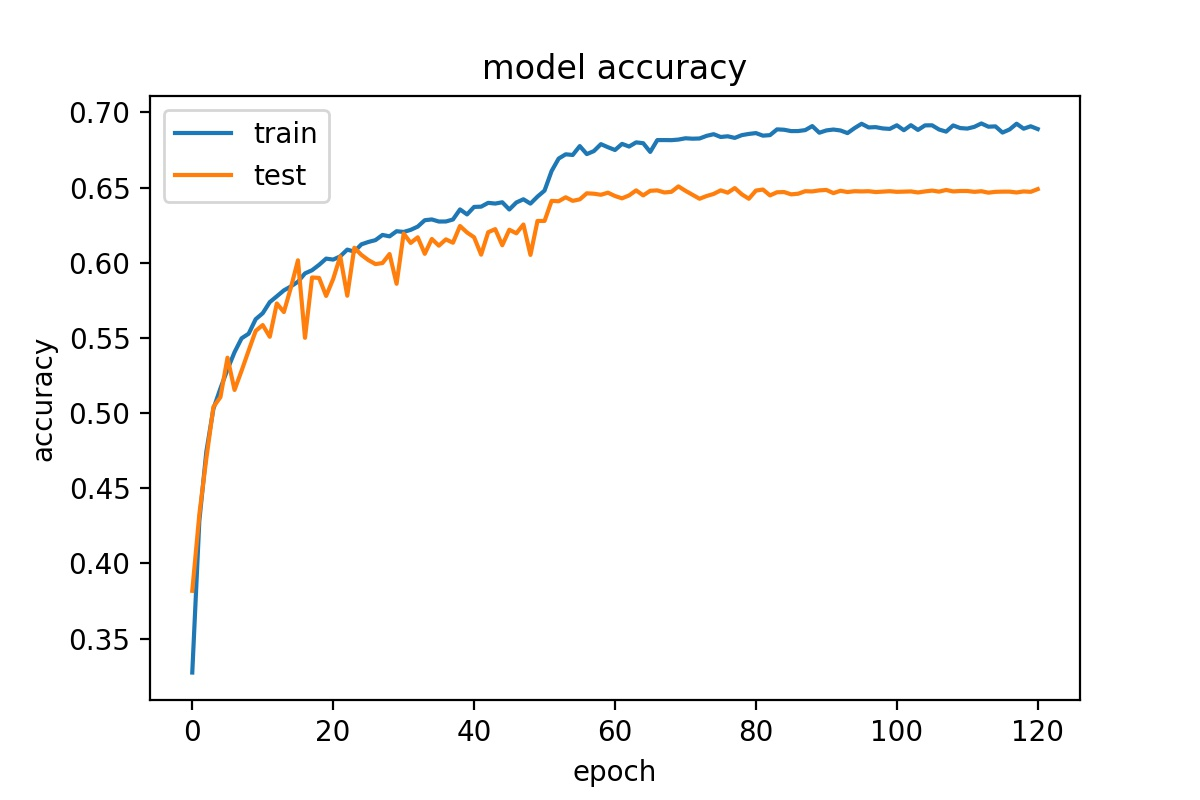
\includegraphics[width=8cm,height=6cm]{images/emotion_acc_2.jpg}
        \caption{Trained model train/test accuracy}
        \label{fig:emoiton_acc_2}
    \end{subfigure}
    \hfill
    \begin{subfigure}[b]{0.5\textwidth}
        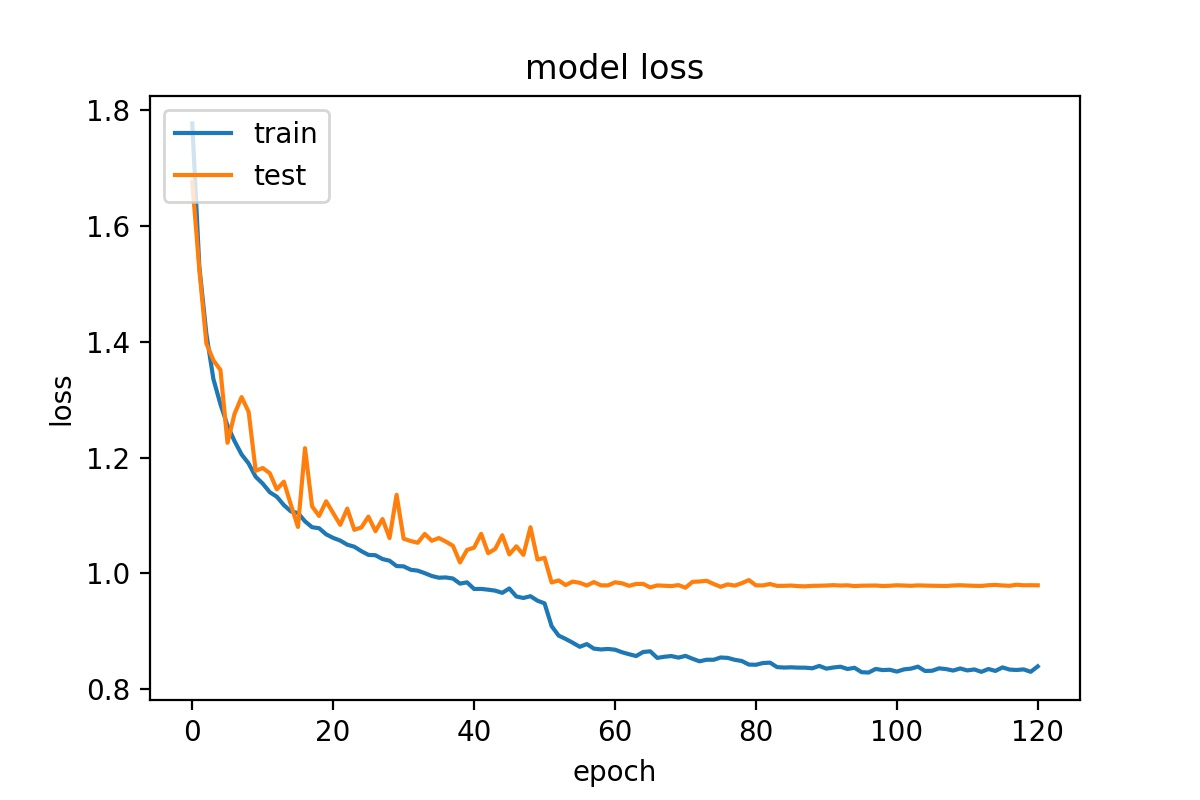
\includegraphics[width=8cm,height=6cm]{images/emotion_loss_2.jpg}
        \caption{Trained model train/test loss}
        \label{fig:emoiton_loss_2}
    \end{subfigure}
    
    \caption{Trained model results}
    \label{fig:emoiton_results_2}
\end{figure}


\textbf{Comparison}: Consider table: \ref{tbl:emotion_comparison}, we held a thorough comparison with every little detail between the two models. We can see clearly how our model overcomes the pre-trained one, in terms of execution time, overfitting, and memory allocation.\\


\begingroup
\centering
\begin{tabular} { | p {4 cm} || p {6 cm} |p {6 cm} |}
    \hline
    \textbf{Compare} & \textbf{Trained model} & \textbf{VGG16 Pre-trained}\\
    \hline
    \hline
    \rule{0pt}{15pt} Model size &  900 KB & 40 MB\\
    \hline
    \rule{0pt}{15pt} Time to Load & 0.4 seconds & 2.8 seconds\\
    \hline
    \rule{0pt}{15pt} Train one epoch & 3 minutes CPU, 15 seconds TPU & 3 hours CPU, 30 minutes GPU\\
    \hline
    \rule{0pt}{15pt} Level of convergence & epoch 60 & never, runs till' overfitting\\
    \hline
    \rule{0pt}{15pt} Train accuracy & 0.7 & 0.88\\
    \hline
    \rule{0pt}{15pt} Test accuracy & 0.66 & 0.65\\
    \hline
    \rule{0pt}{15pt} Suffers overfitting & False & True\\
    \hline
    \rule{0pt}{15pt} Convergence & True & False\\
    \hline
    \rule{0pt}{15pt} Processing 1800 frames & 1.5 minutes & 3.5 minutes\\
    \hline
    \rule{0pt}{15pt} Meaningful results & True & True\\
    \hline
\end{tabular}
\captionof{table}{Emotion detection: Comparing trained model and VGG16}
\label{tbl:emotion_comparison}
\endgroup
\vspace{1cm}

\textbf{Conclusion}: At the end we were happy with the results we got, we kept trying them on different videos with different definitions and different extensions, and results were very acceptable. We decided to keep our trained model for production (merging with the web site) instead of the pre-trained one.






\newpage
\subsection{Module Testing 2: Personality Analysis Agent}
Please refer to module's introduction at section: \ref{sec:module_2} before going deeper in this section! This section is divided into phases, our plan changed couple of times during the implementation and evaluation of our agent.\\


\textbf{Dataset}: We used \href{https://www.kaggle.com/datasnaek/mbti-type}{(\underline{source})} \textit{-Myers Briggs Type Indicator-}, another dataset we could've used set for OCEAN traits, but as we've discussed before \ref{sec:mbti_ls} MBTI traits are more descriptive than OCEAN's, so we settled with them.\\

\textbf{Intuition}: We knew from the start that this particular problem requires sequence models to beat, section \ref{Sequence Models}, we did our research and agreed to implement a very powerful state-of-the-art model using BERT architecture, and then try our best to overcome its results.\\

\textbf{Phase 1: BERT model (pre-trained)}: BERT architecture is massive, and used to solve complex problems \cite{bert}, we were not able to download it locally, so we used it using a server/client channel, send requests through a socket, and receive results, these results are then used for prediction. This approach worked and gave astonishing results, but it consumed a lot of our resources and usually laptops crashed; so we didn't proceed with it.\\

\textbf{Phase 2: BERT embeddings}: We then came to a solution were we only used pre-trained BERT embeddings \textbf{only}, we took them as \textbf{initial} values to our embeddings, trained them with two ANN layers, one for reducing complexity and the other is for prediction. Results were as follows: \ref{fig:bert_2_results}. 

As you can see, right from the start that model is overfitting, the validation accuracy kept oscillating while training accuracy kept overfitting to the dataset and validation loss kept increasing; and that's probably intuitive because of the complexity of our model.

It was trained for 100 epochs, the more epochs it's being trained for the more overfit it became, trained with batch size=64, learning rate = 0.00001, adam optimizer and cross-entropy loss.\\

\begin{figure}[h]
    % \centering
    \begin{subfigure}[b]{0.5\textwidth}
        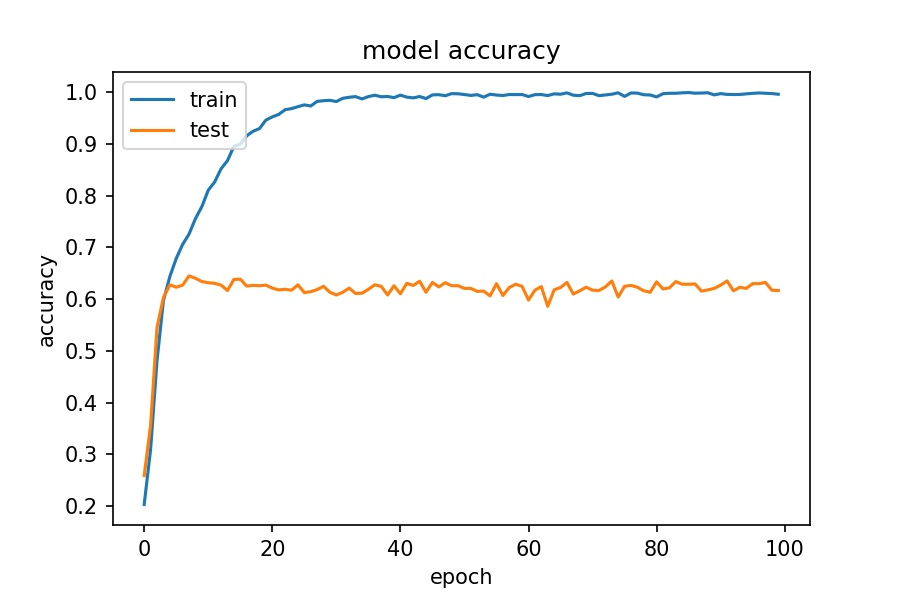
\includegraphics[width=8cm,height=6cm]{images/bert_acc.jpg}
        \caption{BERT + 2ANN model train/test accuracy}
        \label{fig:bert_acc}
    \end{subfigure}
    \hfill
    \begin{subfigure}[b]{0.5\textwidth}
        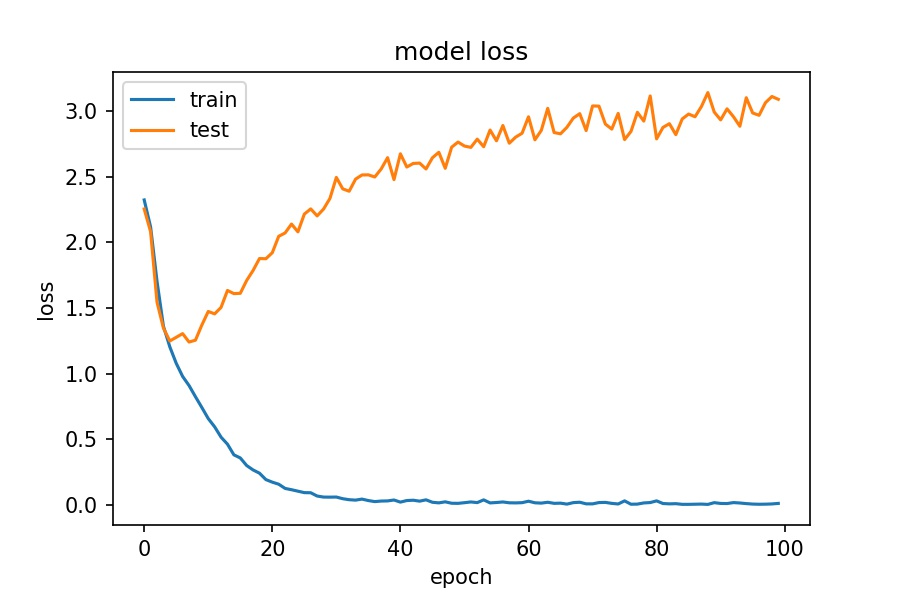
\includegraphics[width=8cm,height=6cm]{images/bert_loss.jpg}
        \caption{BERT + 2ANN model train/test loss}
        \label{fig:bert_loss}
    \end{subfigure}
    
    \caption{BERT + 2ANN model results}
    \label{fig:bert_2_results}
\end{figure}

\textbf{Phase 2: solutions}: We then began to tune the learning rate, results didn't get any better, as a matter of fact reducing the learning rate only made the bad news flies slower. Batch size did the same also, decreasing it made the model overfits slowly.

We had to reduce the level of complexity that we are dealing with, so we trained the model with a higher learning rate, with one less layer of ANN, lower batch size, and for a fewer number of epochs. Results were not much better, real-life examples gave same outcomes and sometimes even worse, so we discarded this modification.

A lot of time was consumed trying to make the best out of this model, until we decided to leave it as is, overfit with some acceptable results on real-life examples.\\

\begin{itemize}
    \item learning rate = 0.0001
    \item batch size = 32
    \item epochs = 50\\
\end{itemize}

\textbf{Phase 3: Analysis and Division}: One important step we had to do before training our own model, and that was visualizing the data. To get inspired; and it did, our dataset was totally biased towards certain classes as you can see in figure \ref{fig:mbti_data_biased}. We needed to limit overcome this issue, so we searched for real-life estimate of how frequent does each trait exist, and transformed our data to be randomly obeying this estimate, figure \ref{fig:mbti_data_biased_2}.


A problem arose from this action: our data became very small; in order to suite classes with fewer examples while obeying traditional estimate. 

So we came up with a good solution: dividing our dataset into four similar ones, to transform the problem into four binary classification smaller problems, with the same small data, creating four classifiers each operating on a certain trait.

We tried many sequence models architectures, with a wide range of different learning rates, hoping to make any advancement, results shown in tables: \ref{tbl:mbti_results_one}, \ref{tbl:mbti_results_two}, and \ref{tbl:mbti_results_three}, we tried three different architectures, with almost the same sizes, same pre-processing, and of course same data, LSTM, simple RNN, and bidirectional RNN.

Results are not the best, it's almost like flipping a coin, but actually it turns out that these four simpler classifiers combined behaves better when it comes to real-life examples, as each model is trying to extract the most context based on the fed dataset.\\

\begin{figure}[h!]
\centering
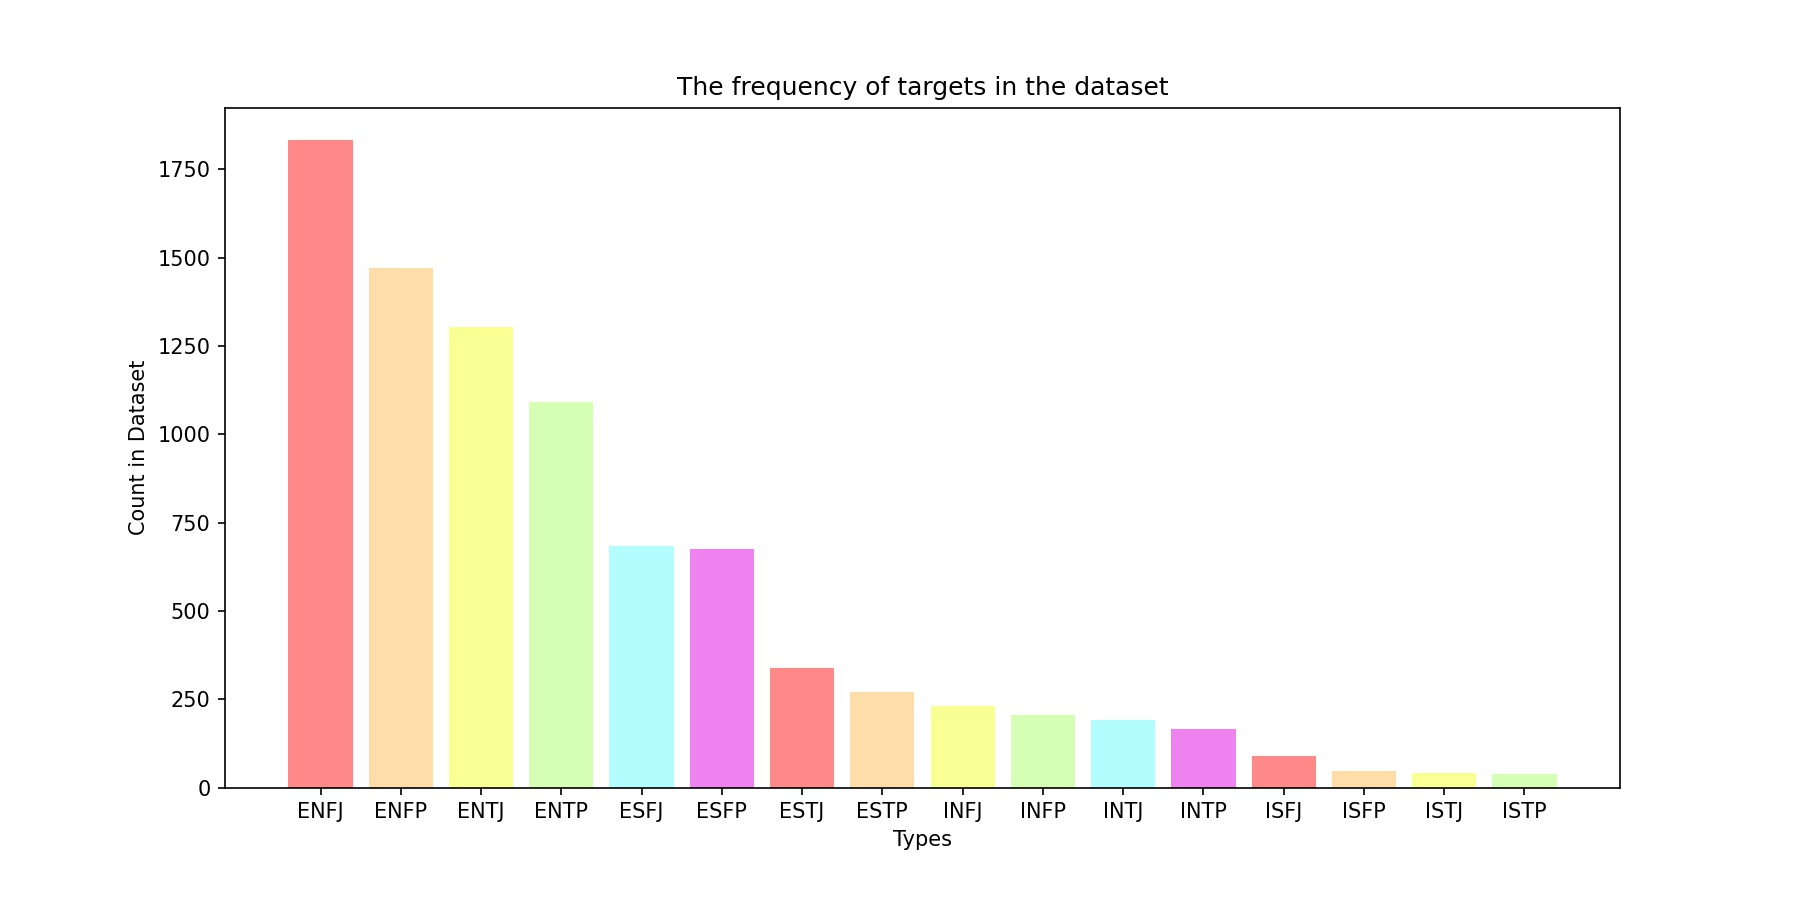
\includegraphics[width=1\textwidth]{images/freq_of_targets.jpg}
\caption{Frequency of targets (biased)}
\label{fig:mbti_data_biased}
\end{figure}

\begin{figure}[h!]
\centering
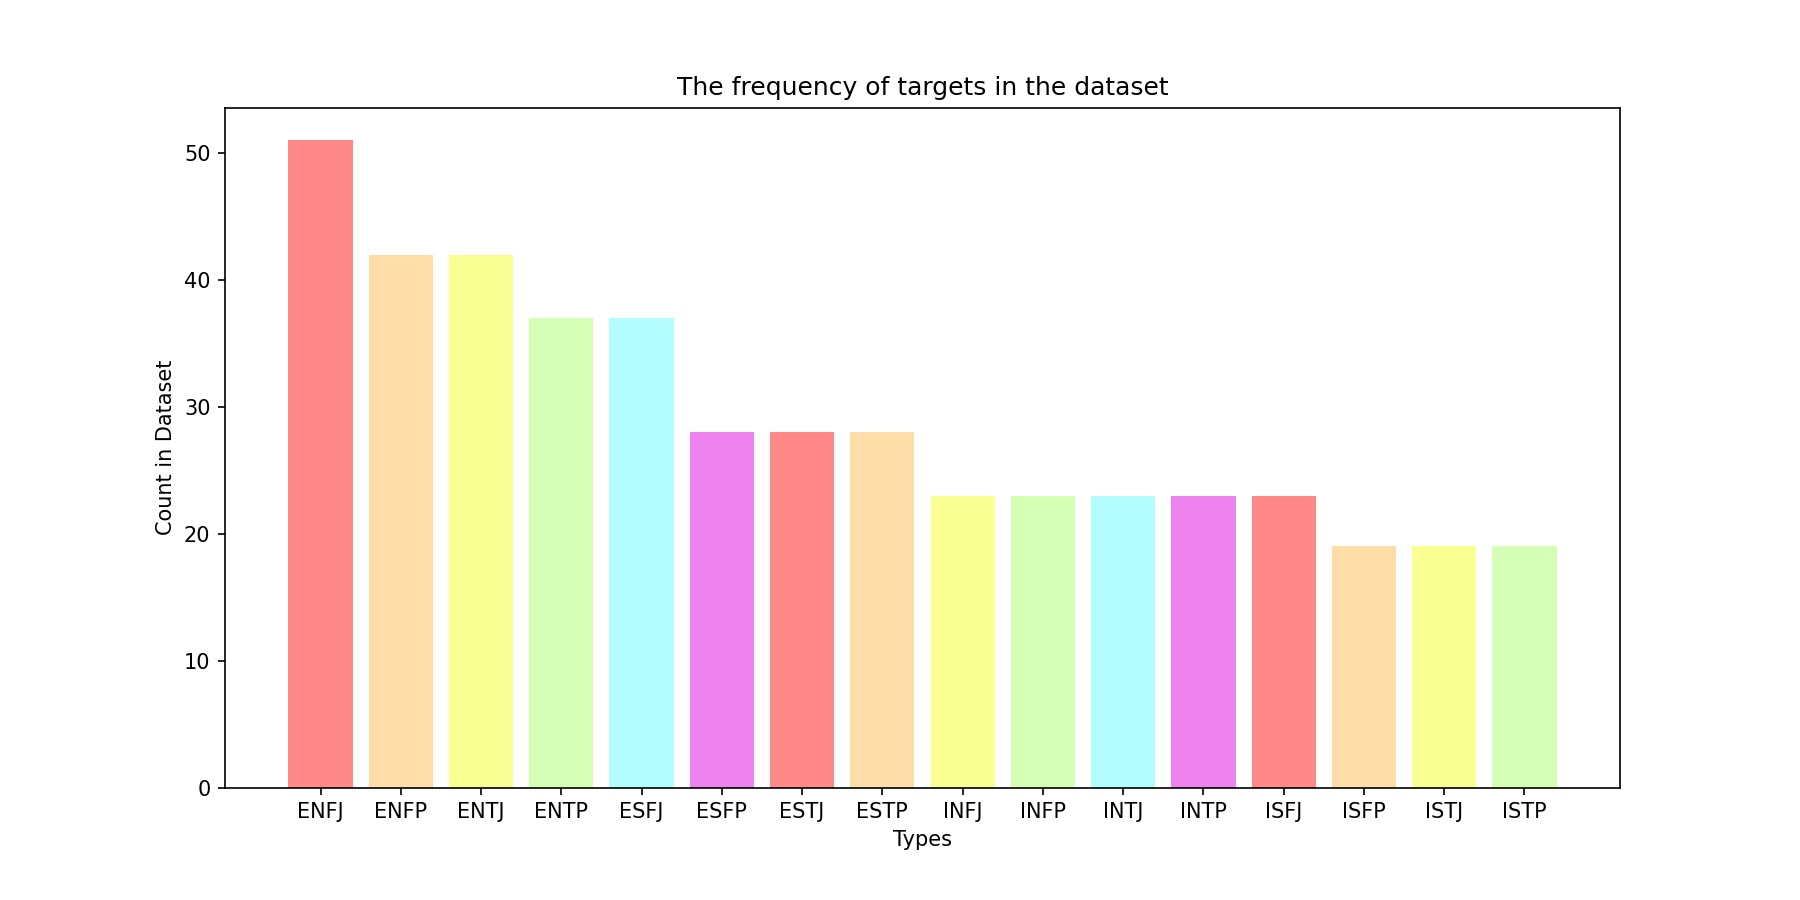
\includegraphics[width=1\textwidth]{images/freq_of_targets_2.jpg}
\caption{Frequency of targets (unbiased)}
\label{fig:mbti_data_biased_2}
\end{figure}



\begingroup
\centering
\begin{tabular} { | p {4 cm} || p {2 cm} |p {2 cm} |p {2 cm} |}
    \hline
    \textbf{Architecture} & \textbf{Learning rate} & \textbf{Classifier} & \textbf{Accuracy}\\
    \hline
    \hline
    \rule{0pt}{15pt} LSTM & 0.01 & F/T & 0.58\\
    \hline
    \rule{0pt}{15pt} LSTM & 0.01 & I/E & 0.49\\
    \hline
    \rule{0pt}{15pt} LSTM & 0.01 & N/S & 0.52\\
    \hline
    \rule{0pt}{15pt} LSTM & 0.01 & P/J & 0.53\\
    \hline
    \rule{0pt}{15pt} LSTM & 0.001 & F/T & 0.44\\
    \hline
    \rule{0pt}{15pt} LSTM & 0.001 & I/E & 0.5\\
    \hline
    \rule{0pt}{15pt} LSTM & 0.001 & N/S & 0.61\\
    \hline
    \rule{0pt}{15pt} LSTM & 0.001 & P/J & 0.44\\
    \hline
    \rule{0pt}{15pt} LSTM & 0.0001 & F/T & 0.53\\
    \hline
    \rule{0pt}{15pt} LSTM & 0.0001 & I/E & 0.5\\
    \hline
    \rule{0pt}{15pt} LSTM & 0.0001 & N/S & 0.59\\
    \hline
    \rule{0pt}{15pt} LSTM & 0.0001 & P/J & 0.66\\
    \hline
    \rule{0pt}{15pt} LSTM & 0.00001 & F/T & 0.53\\
    \hline
    \rule{0pt}{15pt} LSTM & 0.00001 & I/E & 0.55\\
    \hline
    \rule{0pt}{15pt} LSTM & 0.00001 & N/S & 0.59\\
    \hline
    \rule{0pt}{15pt} LSTM & 0.00001 & P/J & 0.66\\
    \hline
\end{tabular}
\captionof{table}{Personality analysis: Four small LSTM binary classifiers.}
\label{tbl:mbti_results_one}
\endgroup
\vspace{1cm}



\begingroup
\centering
\begin{tabular} { | p {4 cm} || p {2 cm} |p {2 cm} |p {2 cm} |}
    \hline
    \textbf{Architecture} & \textbf{Learning rate} & \textbf{Classifier} & \textbf{Accuracy}\\
    \hline
    \hline
    \rule{0pt}{15pt} RNN & 0.01 & F/T & 0.48\\
    \hline
    \rule{0pt}{15pt} RNN & 0.01 & I/E & 0.58\\
    \hline
    \rule{0pt}{15pt} RNN & 0.01 & N/S & 0.59\\
    \hline
    \rule{0pt}{15pt} RNN & 0.01 & P/J & 0.39\\
    \hline
    \rule{0pt}{15pt} RNN & 0.001 & F/T & 0.55\\
    \hline
    \rule{0pt}{15pt} RNN & 0.001 & I/E & 0.48\\
    \hline
    \rule{0pt}{15pt} RNN & 0.001 & N/S & 0.49\\
    \hline
    \rule{0pt}{15pt} RNN & 0.001 & P/J & 0.58\\
    \hline
    
\end{tabular}
\captionof{table}{Personality analysis: Four small RNN binary classifiers.}
\label{tbl:mbti_results_two}
\endgroup
\vspace{1cm}


\begingroup
\centering
\begin{tabular} { | p {4 cm} || p {2 cm} |p {2 cm} |p {2 cm} |}
    \hline
    \textbf{Architecture} & \textbf{Learning rate} & \textbf{Classifier} & \textbf{Accuracy}\\
    \hline
    \hline
    \rule{0pt}{15pt} BI-RNN & 0.01 & F/T & 0.5\\
    \hline
    \rule{0pt}{15pt} BI-RNN & 0.01 & I/E & 0.43\\
    \hline
    \rule{0pt}{15pt} BI-RNN & 0.01 & N/S & 0.48\\
    \hline
    \rule{0pt}{15pt} BI-RNN & 0.01 & P/J & 0.61\\
    \hline
    \rule{0pt}{15pt} BI-RNN & 0.001 & F/T & 0.46\\
    \hline
    \rule{0pt}{15pt} BI-RNN & 0.001 & I/E & 0.44\\
    \hline
    \rule{0pt}{15pt} BI-RNN & 0.001 & N/S & 0.6\\
    \hline
    \rule{0pt}{15pt} BI-RNN & 0.001 & P/J & 0.38\\
    \hline
    
\end{tabular}
\captionof{table}{Personality analysis: Four small Bi-RNN binary classifiers.}
\label{tbl:mbti_results_three}
\endgroup
\vspace{1cm}


\textbf{Phase 4: Limits}: We got stuck for a while, reading articles and trying to come up with new plans, some of them were total failure -we didn't even bother mention them here-, until we figured that this exact problem is not yet to be solved, and has no upper ceiling to exceed \cite{state_of_the_art_pers_text}. So we developed another model, with bidirectional LSTM, learning rate = 0.001, and embedding vector size=100, trying to make it reach the best outcome there is (ie. 66\%), but again we failed to beat it, as a matter of fact our model overfits worse than BERT pre-trained, and BERT initialized models. Achieving training accuracy near perfect (0.99) and validation accuracy (0.2).\\

\textbf{Conclusion}: At the end we decided to keep the second phase model, with BERT embeddings used as an initialization to our model, with two ANN layers after that; due to its good sensing results in real-life examples, compared to other models.






\newpage
\subsection{Module Testing 3: Resume Ranker Agent}
Please refer to module's introduction at section: \ref{sec:module_3} before going deeper in this section!\\

\textbf{First impression}: This is a brand new problem, that had no previous solid related work that we could rely on, doing our research we came to a decision that we will not use an AI model (sequence model) to solve this issue, and only treating it as query/document search problem, but then realized that \textit{resumes} capture contextual meanings that needed to be exploited; so we implemented word2vec model for that purpose.\\

\textbf{Dataset}: We were able to find two different sources for dataset, the first was held by Kaggle platform \href{https://www.kaggle.com/ranaelmahmoudy/curriculum-vitae-data-pdf}{(\underline{source})} contains only resumes in \textit{pdf} and \textit{docx} formats, unsupervised dataset with only resumes with no matching to any job description, consists of 4500 resumes, with nearly 20 of them corrupted. The second dataset we found was from unknown \href{https://drive.google.com/file/d/17M9oDPip5JFFFNJhDCBQKy8BMqoyxajU/view}{(\underline{source})} collected for a school project found on github, so we held it for testing purposes, this dataset contains resumes and matching job descriptions in different fields (finance, trust, managing ..etc.)\\

\textbf{Test}: Since this is an unsupervised problem, we needed to create tests to indicate how far is our model correct, so we created three tailored tests, where it contains two folders: one contains the job description, and the second contains 60 resumes, 30 of them matches the job description, and the other 30 does not. These three tests were held on three different fields: Trust/Accounting/Managing.\\

\textbf{Choice of model}: At first we were not sure what to use in order to create our model, we thought obviously for \textit{clustering}, but then figured that we are not using information stored in \textit{job description} at all, so we settled on training word embeddings matrix using resumes and \textit{rank} them according to best matching ones with the job description. Therefore we went with word2vec and glove models.\\

\textbf{Pre-trained}: We used \textit{gensim} library with its helpful toolkit to create models and also download pre-trained ones for establishing clear ground truth to our work. We picked \textit{glove-wiki-gigaword-100} pre-trained model to test with. this model -which we'll call "wiki"- contains a vocabulary of size $400,000$ unique words, each represented with vector size = 100, trained using \textit{glove} architecture on Wikipedia dataset.\\

\textbf{Evaluation}: Now that we have a pre-trained model with dataset, we needed to establish an evaluation function to make use of the information in hand, so we came up with two different ranking techniques discussed at \ref{sec:ranker}. Storing results in ".csv" files and then calculates \textit{F1-score} for these results; the intuition behind this approach is that we have True/False examples, with false positives (negative examples predicted as true) and false negatives (positive examples predicted as false). Equation goes as follows \ref{eq:f1_score}:

\begin{equation} \label{eq:f1_score}
F_1 = \frac{TP}{TP + \frac{1}{2}(FP + FN)}
\end{equation}
\myequations{F1 Score}


TP: number of true positive examples.\\

FP: number of false positive examples.\\

FN: number of false negative examples.\\

We set the mean (average) of \textit{cosine} values to be the threshold for positive/negative examples; since we have 30/30 true/false examples. This figure \ref{fig:resume_results_1} may illustrate better.\\

\begin{figure}[h!]
\centering
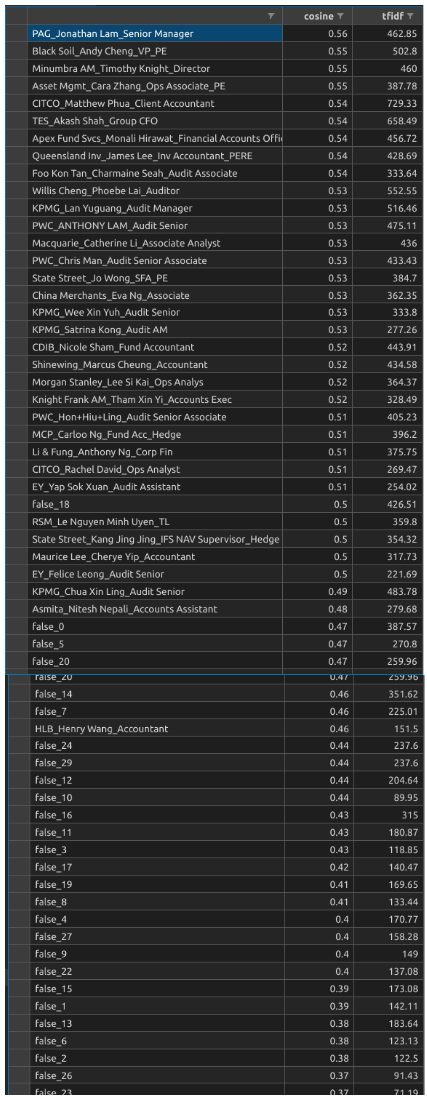
\includegraphics[width=0.6\textwidth]{images/resume_results_1.png}
\caption{Resume ranker result example}
\label{fig:resume_results_1}
\end{figure}

\textbf{Pre-trained results}: In the following table is the pre-trained model "wiki" results on three different tests (stated before), table \ref{tbl:resume_results_1}. Note that, because number of false examples equals the number of true examples, f1 score is reduced to simple accuracy estimation (number of true positives / number of all positives).\\


\begingroup
\centering
\begin{tabular} { | p {4 cm} || p {2 cm} | p {2 cm} |p {2 cm} |p {2 cm} |}
    \hline
    \textbf{Test id} & \textbf{TP} & \textbf{FP} & \textbf{FN}& \textbf{$F_1$} score\\
    \hline
    
    \hline
    \rule{0pt}{15pt} Asst. Finance &  19 & 11 & 11 & 0.6333\\
    \hline
    \rule{0pt}{15pt} Manager &23 & 7 & 7 & 0.766\\
    \hline
    \rule{0pt}{15pt} Trust administrator & 22 & 8 & 8 & 0.73\\
    \hline
    
\end{tabular}
\captionof{table}{Resume ranker pre-trained model results}
\label{tbl:resume_results_1}
\endgroup
\vspace{1cm}

\textbf{Actual model}: We used \textit{word2vec} model implemented by \textbf{gensim} library, fed it parsed data (resumes) creating a vocabulary of size $63611$ unique words.\\

\textbf{Issues}: One issue we had when first started tuning our model, and that it was tested with only true samples and cosine similarity, so we faced overfitting when we increased the vector size representing our words. However, we figured it out, and designed our tests as discussed before.\\

\textbf{Tuning}: Now that every thing is ready, we had three main hyperparameters to tune: learning rate, vector size, and window size. In addition to the training model used (skip-gram or CBOW). We decided to use skip-gram because the type of problem is requiring the prediction of surrounding words given the center word. Below is reporting table with different sizes, epochs, and learning rates against f1 scores, table \ref{tbl:resume_results_2}. Each training trial would take from 30 to 60 minutes on average.\\



\begingroup
\centering
\begin{tabular} { | p {2 cm} || p {2 cm}  | p {2 cm} |p {2 cm} |}
    \hline
    \textbf{f1 score} & \textbf{LR} & \textbf{vector size}& \textbf{window size}\\
    \hline
    
    \hline
    \rule{0pt}{15pt} 0.533 &  0.01 & 100 & 5\\
    \hline
    \rule{0pt}{15pt} 0.867 &0.0001 & 100 & 1\\
    \hline
    \rule{0pt}{15pt} 0.6  & 0.0001 & 100 & 2\\
    \hline
    \rule{0pt}{15pt} 0.633 & 0.0001 & 100 & 4\\
    \hline
    \rule{0pt}{15pt} 0.7 &0.0001 & 300 & 9\\
    \hline
    \rule{0pt}{15pt} 0.967 & 0.001 & 300 & 15\\
    \hline
    
\end{tabular}
\captionof{table}{Resume ranker pre-trained model results}
\label{tbl:resume_results_2}
\endgroup
\vspace{1cm}


\textbf{Final settings}: At last we settled on these parameters, tuned for 150 epochs:
\begin{itemize}
    \item learning rate: 0.001
    \item vector size: 300
    \item window size: 15\\
\end{itemize}

\textbf{Comparison}: Clearly our trained model behaves better in terms of training and also real time production, below is a thorough comparison between the two models, tested on the same environment, table \ref{tbl:resume_results_3}.\\


\begingroup
\centering
\begin{tabular} { | p {5 cm} || p {5 cm} |p {5 cm} |}
    \hline
    \textbf{Compare} & \textbf{Trained model} & \textbf{Pre-trained wiki}\\
    \hline
    \hline
    \rule{0pt}{15pt} Model size &  325 MB & 500 MB\\
    \hline
    \rule{0pt}{15pt} Time to Load & 5.1 seconds & 40 seconds\\
    \hline
    \rule{0pt}{15pt} Train one epoch & 30 minutes CPU & didn't require training\\
    \hline
    \rule{0pt}{15pt} Overall accuracy & 0.9 & 0.7\\
    \hline
    \rule{0pt}{15pt} Suffers overfitting & False & False\\
    \hline
    \rule{0pt}{15pt} Processing 60 resumes & 50 seconds & 60 seconds\\
    \hline
    \rule{0pt}{15pt} Meaningful results & True & True\\
    \hline
    \rule{0pt}{15pt} Vocabulary size & 63,611 & 400,000\\
    \hline
    \rule{0pt}{15pt} Vector size & 300 & 100\\
    \hline
\end{tabular}
\captionof{table}{Resume ranker: Comparing trained model and glove wiki}
\label{tbl:resume_results_3}
\endgroup
\vspace{1cm}

\textbf{Conclusion}: At the end, we were able to reach our roof by training \textit{word2vec} model with our data, achieving higher scores as we hoped, this is pretty reasonable and intuitive; our model is trained on jobs-related subjects, rather than random information from the "wiki"; that's why our model behaves better, even with unseen data.\\

\newpage
\subsection{Back-end API Testing}
We used \href{https://www.postman.com/}{\underline{Postman}} to test the API (application programming interface) independently without the existence of the client side (front-end); by sending requests and ensuring that we get the expected responses.

\subsection{Distributing Requests}
\label{sec:distributing_requests}
We tried to run multiple back-end master nodes to distribute the clients' requests among them using a load balancer, explained at section \ref{sec:Load}. 
We implemented a \textit{round robin} load balancer using Node.js, that receives a request, decomposes it, and sends it back to one of the connected nodes in a circular order.

We compared the performance with \href{https://www.nginx.com/}{\underline{NGINX}} web server, by testing the request of getting some jobs and using 3 back-end nodes. We used \href{http://manpages.ubuntu.com/manpages/bionic/man1/ab.1.html}{\underline{Apache}} benchmark tool to send requests to the server. 
By running the following command:
\begin{verbatim}
ab -c 10 -n 10000 http://localhost/api/job    
\end{verbatim}
It sends 10000 requests to the given endpoint, each 10 of them are sent concurrently.
We obtained the following results: \\



\begingroup
\centering
\begin{tabular} { | p {5 cm} || p {3.33 cm} |p {3.33 cm} | p{3.34 cm} | }
    \hline
    \textbf{Compare} & \textbf{Single node} & \textbf{Implemented load balancer} & \textbf{NGINX}\\
    \hline
    \hline
    \rule{0pt}{15pt} Time taken for tests &  30 seconds & 37 seconds & 27 seconds\\
    \hline
    \rule{0pt}{15pt} Requests per second & 330.5  & 270 & 370 \\
    \hline
    \rule{0pt}{15pt} Mean time per request & 30 ms & 37 ms & 27 ms\\
    \hline
    \rule{0pt}{15pt} Mean time per request across all concurrent requests & 3 ms & 3.7 ms & 2.7 ms \\
    \hline
    
\end{tabular}
\captionof{table}{Load balancer: compare implemented load balancer with nginx}
\label{tbl:load_balancer_resutls}
\endgroup
\vspace{1cm}
It's obvious that our implemented load balancer performance is worse than the performance of a single node, because of the overhead of decomposing incoming request and sending it again to another server. 
NGINX performance is better than using only a single node.
\newpage

\subsection{Integration Testing}
\label{sec:integration_test}
After testing each module separately (three agents, worker, front-end, and back-end), we began to design thorough tests that span the whole project entirely, we started with simpler phases of the application and began to append one module at a time.

Steps were as follows:
\begin{enumerate}
    \item Testing the application without intelligent agents.
    \item Appending one agent at a time.
    \item Testing the whole system without distributing the work load among workers.
    \item Distributing work loads among multiple workers, ONE machine.
    \item Distributing work loads among multiple workers, separate machines.
\end{enumerate}


\textbf{Testing the application without intelligent agents}: We made sure that every \textit{request} is working correctly and the \textit{feedback} (response) is sent back to the user in the front-end. Tests applied at this phase were mainly made for verification purposes only, no heavy processing were yet made to be tested, only the platform that we will be using; thus tests were made with dummy inputs.\\

\textbf{Appending one agent at a time}: To ensure that each agent (model) works perfectly, it was tested locally first (see previous sections for more), then we appended them one at a time to our web application, executing them with only one worker, that its job was to make sure that agents executes properly with real inputs and  meaningful results.\\
We started with \textit{emotion detection} agent, then added \textit{resume ranker} agent, and finished with \textit{personality analysis} agent. Each one of them was tested with one worker, making sure that it executes properly and with no naming conflicts in case of multiple inputs with the same data was sent; we solved this issue by naming data with two distinctive ids, the first is the job description and the second is user's id, thus if a user tried to apply for another job with the same data, names will be different across multiple machines and even if they were processed on one machine.\\

\textbf{Testing the whole system without distributing the work load among workers}: We created an admin, an HR, and multiple applicants, the HR created some jobs, and applicants applied for the created jobs, their videos and textual answers were sent to the workers to be processed and then the HR disabled applying for the job anymore and requested to analyze the given resumes. The results were sent back from the workers to the back-end and the HR was able to see the ranked applicants and their analyzed information. All of this was executed using one worker only, time was logged for reporting later.\\

\textbf{Distributing work loads among multiple workers, ONE machine} Then we applied same tests as above but with distributing the work load among multiple workers (three of them) that worked in parallel (concurrently) locally on one machine.\\

\textbf{Distributing work loads among multiple workers, separate machine} At last we applied the same test on multiple separate machines, connected via the internet, each has one worker that's fully operating alone on the system (ie. full capacity).\\

Finally we compare the timing performance between executing tasks using one worker (no distribution) and three workers locally distributed (one machine) and separate distributed machines. 

Testing setup was:
\begin{itemize}
    \item Two jobs created by different interviewers.
    \item Three applicants applying for both of them.
    \item All jobs require video.
    \item First job requires answering three questions, and the second requires five questions.
\end{itemize}
We obtained the following results:\\

\begingroup
\centering
\begin{tabular} { | p {3 cm} || p {4 cm} |p {4 cm} |p {4 cm} | }
    \hline
    \textbf{Compare} & \textbf{One Worker} & \textbf{Three Workers} & \textbf{Distributed Workers} \\
    \hline
    \hline
    \rule{0pt}{15pt} Time taken & 30 minutes & 25 minutes & 15 minutes\\
    \hline
    
\end{tabular}
\captionof{table}{Integration testing: comparing 1 worker against 3 (distributed)}
\label{tbl:integration_testing_resutls}
\endgroup
\vspace{1cm}

One last thing to mention is that when the case of multiple workers on one machine, error rate becomes larger, as one machine can't handle all this processing at once, so we had to repeat the same test until one of them passed.\\


\section{Testing Schedule}
We were testing the separate modules while developing them, and the integration testing was done after we finished all the modules. The testing and validation of the AI models took a lot of time. The emotion detection module took 10 hours. The personality analysis module took approximately 5 days. The resume ranker module took 2 days.

% \section{Comparative Results to Previous Work}
